% Options for packages loaded elsewhere
\PassOptionsToPackage{unicode}{hyperref}
\PassOptionsToPackage{hyphens}{url}
%
\documentclass[
  11pt,
  ignorenonframetext,
]{beamer}
\usepackage{pgfpages}
\setbeamertemplate{caption}[numbered]
\setbeamertemplate{caption label separator}{: }
\setbeamercolor{caption name}{fg=normal text.fg}
\beamertemplatenavigationsymbolsempty
% Prevent slide breaks in the middle of a paragraph
\widowpenalties 1 10000
\raggedbottom
\setbeamertemplate{part page}{
  \centering
  \begin{beamercolorbox}[sep=16pt,center]{part title}
    \usebeamerfont{part title}\insertpart\par
  \end{beamercolorbox}
}
\setbeamertemplate{section page}{
  \centering
  \begin{beamercolorbox}[sep=12pt,center]{part title}
    \usebeamerfont{section title}\insertsection\par
  \end{beamercolorbox}
}
\setbeamertemplate{subsection page}{
  \centering
  \begin{beamercolorbox}[sep=8pt,center]{part title}
    \usebeamerfont{subsection title}\insertsubsection\par
  \end{beamercolorbox}
}
\AtBeginPart{
  \frame{\partpage}
}
\AtBeginSection{
  \ifbibliography
  \else
    \frame{\sectionpage}
  \fi
}
\AtBeginSubsection{
  \frame{\subsectionpage}
}
\usepackage{amsmath,amssymb}
\usepackage{iftex}
\ifPDFTeX
  \usepackage[T1]{fontenc}
  \usepackage[utf8]{inputenc}
  \usepackage{textcomp} % provide euro and other symbols
\else % if luatex or xetex
  \usepackage{unicode-math} % this also loads fontspec
  \defaultfontfeatures{Scale=MatchLowercase}
  \defaultfontfeatures[\rmfamily]{Ligatures=TeX,Scale=1}
\fi
\usepackage{lmodern}
\usetheme[]{metropolis}
\ifPDFTeX\else
  % xetex/luatex font selection
\fi
% Use upquote if available, for straight quotes in verbatim environments
\IfFileExists{upquote.sty}{\usepackage{upquote}}{}
\IfFileExists{microtype.sty}{% use microtype if available
  \usepackage[]{microtype}
  \UseMicrotypeSet[protrusion]{basicmath} % disable protrusion for tt fonts
}{}
\makeatletter
\@ifundefined{KOMAClassName}{% if non-KOMA class
  \IfFileExists{parskip.sty}{%
    \usepackage{parskip}
  }{% else
    \setlength{\parindent}{0pt}
    \setlength{\parskip}{6pt plus 2pt minus 1pt}}
}{% if KOMA class
  \KOMAoptions{parskip=half}}
\makeatother
\usepackage{xcolor}
\newif\ifbibliography
\usepackage{color}
\usepackage{fancyvrb}
\newcommand{\VerbBar}{|}
\newcommand{\VERB}{\Verb[commandchars=\\\{\}]}
\DefineVerbatimEnvironment{Highlighting}{Verbatim}{commandchars=\\\{\}}
% Add ',fontsize=\small' for more characters per line
\newenvironment{Shaded}{}{}
\newcommand{\AlertTok}[1]{\textcolor[rgb]{1.00,0.00,0.00}{\textbf{#1}}}
\newcommand{\AnnotationTok}[1]{\textcolor[rgb]{0.38,0.63,0.69}{\textbf{\textit{#1}}}}
\newcommand{\AttributeTok}[1]{\textcolor[rgb]{0.49,0.56,0.16}{#1}}
\newcommand{\BaseNTok}[1]{\textcolor[rgb]{0.25,0.63,0.44}{#1}}
\newcommand{\BuiltInTok}[1]{\textcolor[rgb]{0.00,0.50,0.00}{#1}}
\newcommand{\CharTok}[1]{\textcolor[rgb]{0.25,0.44,0.63}{#1}}
\newcommand{\CommentTok}[1]{\textcolor[rgb]{0.38,0.63,0.69}{\textit{#1}}}
\newcommand{\CommentVarTok}[1]{\textcolor[rgb]{0.38,0.63,0.69}{\textbf{\textit{#1}}}}
\newcommand{\ConstantTok}[1]{\textcolor[rgb]{0.53,0.00,0.00}{#1}}
\newcommand{\ControlFlowTok}[1]{\textcolor[rgb]{0.00,0.44,0.13}{\textbf{#1}}}
\newcommand{\DataTypeTok}[1]{\textcolor[rgb]{0.56,0.13,0.00}{#1}}
\newcommand{\DecValTok}[1]{\textcolor[rgb]{0.25,0.63,0.44}{#1}}
\newcommand{\DocumentationTok}[1]{\textcolor[rgb]{0.73,0.13,0.13}{\textit{#1}}}
\newcommand{\ErrorTok}[1]{\textcolor[rgb]{1.00,0.00,0.00}{\textbf{#1}}}
\newcommand{\ExtensionTok}[1]{#1}
\newcommand{\FloatTok}[1]{\textcolor[rgb]{0.25,0.63,0.44}{#1}}
\newcommand{\FunctionTok}[1]{\textcolor[rgb]{0.02,0.16,0.49}{#1}}
\newcommand{\ImportTok}[1]{\textcolor[rgb]{0.00,0.50,0.00}{\textbf{#1}}}
\newcommand{\InformationTok}[1]{\textcolor[rgb]{0.38,0.63,0.69}{\textbf{\textit{#1}}}}
\newcommand{\KeywordTok}[1]{\textcolor[rgb]{0.00,0.44,0.13}{\textbf{#1}}}
\newcommand{\NormalTok}[1]{#1}
\newcommand{\OperatorTok}[1]{\textcolor[rgb]{0.40,0.40,0.40}{#1}}
\newcommand{\OtherTok}[1]{\textcolor[rgb]{0.00,0.44,0.13}{#1}}
\newcommand{\PreprocessorTok}[1]{\textcolor[rgb]{0.74,0.48,0.00}{#1}}
\newcommand{\RegionMarkerTok}[1]{#1}
\newcommand{\SpecialCharTok}[1]{\textcolor[rgb]{0.25,0.44,0.63}{#1}}
\newcommand{\SpecialStringTok}[1]{\textcolor[rgb]{0.73,0.40,0.53}{#1}}
\newcommand{\StringTok}[1]{\textcolor[rgb]{0.25,0.44,0.63}{#1}}
\newcommand{\VariableTok}[1]{\textcolor[rgb]{0.10,0.09,0.49}{#1}}
\newcommand{\VerbatimStringTok}[1]{\textcolor[rgb]{0.25,0.44,0.63}{#1}}
\newcommand{\WarningTok}[1]{\textcolor[rgb]{0.38,0.63,0.69}{\textbf{\textit{#1}}}}
\usepackage{graphicx}
\makeatletter
\def\maxwidth{\ifdim\Gin@nat@width>\linewidth\linewidth\else\Gin@nat@width\fi}
\def\maxheight{\ifdim\Gin@nat@height>\textheight\textheight\else\Gin@nat@height\fi}
\makeatother
% Scale images if necessary, so that they will not overflow the page
% margins by default, and it is still possible to overwrite the defaults
% using explicit options in \includegraphics[width, height, ...]{}
\setkeys{Gin}{width=\maxwidth,height=\maxheight,keepaspectratio}
% Set default figure placement to htbp
\makeatletter
\def\fps@figure{htbp}
\makeatother
\setlength{\emergencystretch}{3em} % prevent overfull lines
\providecommand{\tightlist}{%
  \setlength{\itemsep}{0pt}\setlength{\parskip}{0pt}}
\setcounter{secnumdepth}{-\maxdimen} % remove section numbering
\ifLuaTeX
  \usepackage{selnolig}  % disable illegal ligatures
\fi
\IfFileExists{bookmark.sty}{\usepackage{bookmark}}{\usepackage{hyperref}}
\IfFileExists{xurl.sty}{\usepackage{xurl}}{} % add URL line breaks if available
\urlstyle{same}
\hypersetup{
  pdftitle={Análisis de estabilidad y R\_0},
  pdfauthor={Gerardo Martín},
  hidelinks,
  pdfcreator={LaTeX via pandoc}}

\title{Análisis de estabilidad y \(R_0\)}
\subtitle{Ecología teórica}
\author{Gerardo Martín}
\date{28-08-2023}

\begin{document}
\frame{\titlepage}

\hypertarget{el-modelo-sir-con-dinuxe1mica-poblacional}{%
\section{\texorpdfstring{El modelo \(SIR\) con dinámica
poblacional}{El modelo SIR con dinámica poblacional}}\label{el-modelo-sir-con-dinuxe1mica-poblacional}}

\hypertarget{las-ecuaciones}{%
\subsection{Las ecuaciones}\label{las-ecuaciones}}

\begin{frame}{Las ecuaciones}
\begin{align}
  \dot{S} & =\mu - \beta S I - \mu S\\
  \dot{I} & = \beta S I  - (\mu + \gamma) I \\
  \dot{R} & = \gamma I - \mu R
\end{align}

\[\dot{N} = dN / dt\]

\[ N = S + I + R = 1\]
\end{frame}

\hypertarget{condiciones-para-distribuciuxf3n-de-equilibrio}{%
\subsection{Condiciones para distribución de
equilibrio}\label{condiciones-para-distribuciuxf3n-de-equilibrio}}

\begin{frame}{Condiciones para distribución de equilibrio}
Igualamos la ecuación para \(\dot{I} = 0\):

\[\beta SI - (\mu + \gamma)I = 0\]

Factorizando \(I\), tenemos:

\[I(\beta S - (\mu + \gamma))=0\]
\end{frame}

\hypertarget{condiciones-para-distribuciuxf3n-de-equilibrio-1}{%
\subsection{Condiciones para distribución de
equilibrio}\label{condiciones-para-distribuciuxf3n-de-equilibrio-1}}

\begin{frame}{Condiciones para distribución de equilibrio}
Con lo que hay dos soluciones evidentes:

\begin{align}
I^* & = 0\\
S^* & = \frac{\mu + \gamma}{\beta}\\
\end{align}

\begin{enumerate}
\tightlist
\item
  El equilibrio libre de enfermedad (\(I^*\))
\item
  El equilibrio endémico (\(S^*\))
\end{enumerate}
\end{frame}

\hypertarget{relaciuxf3n-con-r_0}{%
\subsection{\texorpdfstring{Relación con
\(R_0\)}{Relación con R\_0}}\label{relaciuxf3n-con-r_0}}

\begin{frame}{Relación con \(R_0\)}
La ecuación para \(R_0\):

\[R_0 = \frac{\beta}{\gamma + \mu}\]

Por lo que:

\[S^* = \frac{1}{R_0}\]
\end{frame}

\hypertarget{la-distribuciuxf3n-de-equilibrio-estable}{%
\subsection{La distribución de equilibrio
estable}\label{la-distribuciuxf3n-de-equilibrio-estable}}

\begin{frame}{La distribución de equilibrio estable}
\begin{itemize}
\item
  Cuando hay infecciones, el nivel de susceptibles será \(S^*\)
\item
  Para encontrar la fracción de infectados, sustituimos \(S^* = 1/R_0\)
  en:
\end{itemize}

\[\mu - \beta S I - \mu S = 0\]

de donde resolvemos para \(I\), obteniendo:

\[I^* = \frac{\mu}{\beta}(R_0 - 1)\]
\end{frame}

\hypertarget{encontrando-r}{%
\subsection{\texorpdfstring{Encontrando
\(R^*\)}{Encontrando R\^{}*}}\label{encontrando-r}}

\begin{frame}{Encontrando \(R^*\)}
Tomando en cuenta que:

\[S^* + I^* + R^* = 1\] y que por lo tanto:

\[R^* = 1 - S^* - I^*\]

Sustituimos \(S^*\) e \(I^*\)
\end{frame}

\hypertarget{la-distribuciuxf3n-del-equilibrio-enduxe9mico}{%
\subsection{La distribución del equilibrio
endémico}\label{la-distribuciuxf3n-del-equilibrio-enduxe9mico}}

\begin{frame}{La distribución del equilibrio endémico}
\[R^* = 1 - \frac{1}{R_0} - \frac{\mu}{\beta}(R_0-1)\]

Tenemos entonces que:

\[(S^*, I^*, R^*) = \left( \frac{1}{R_0}, \frac{\mu}{\beta}(R_0 - 1), 1 - \frac{1}{R_0} - \frac{\mu}{\beta}(R_0-1)\right)\]
\end{frame}

\hypertarget{interpretaciuxf3n-de-condiciones-de-equilibrio}{%
\section{Interpretación de condiciones de
equilibrio}\label{interpretaciuxf3n-de-condiciones-de-equilibrio}}

\hypertarget{en-el-modelo-sir-con-dinuxe1micas}{%
\subsection{\texorpdfstring{En el modelo \(SIR\) con
dinámicas}{En el modelo SIR con dinámicas}}\label{en-el-modelo-sir-con-dinuxe1micas}}

\begin{frame}{En el modelo \(SIR\) con dinámicas}
\begin{itemize}
\item
  Oscilaciones
\item
  Decrecen con tiempo
\item
  Amplitud disminuye
\item
  Período aumenta
\end{itemize}
\end{frame}

\hypertarget{simulaciuxf3n}{%
\subsection{Simulación}\label{simulaciuxf3n}}

\begin{frame}{Simulación}
Valores de parámetros y condiciones iniciales:

\begin{itemize}
\item
  \(1/\mu = 70\) años
\item
  \(\beta = 520\) por año
\item
  \(1/\gamma = 7\) días
\item
  \(S(0) = 0.1\) y \(I(0) = 2.5 \times 10^{-4}\)
\item
  \(R_0 \approx 10\) (para cálculo hay que homogeneizar unidades de
  parámetros)
\end{itemize}
\end{frame}

\hypertarget{cuxf3digo-de-desolve}{%
\subsection{\texorpdfstring{Código de
\texttt{deSolve}}{Código de deSolve}}\label{cuxf3digo-de-desolve}}

\begin{frame}[fragile]{Código de \texttt{deSolve}}
\begin{Shaded}
\begin{Highlighting}[]
\NormalTok{parms }\OtherTok{\textless{}{-}} \FunctionTok{list}\NormalTok{(}
  \AttributeTok{mu =} \DecValTok{1}\SpecialCharTok{/}\NormalTok{(}\DecValTok{70} \SpecialCharTok{*} \DecValTok{365}\NormalTok{),}
  \AttributeTok{beta =} \DecValTok{520} \SpecialCharTok{/} \DecValTok{365}\NormalTok{,}
  \AttributeTok{gamma =} \DecValTok{1}\SpecialCharTok{/}\DecValTok{7}
\NormalTok{)}

\NormalTok{y }\OtherTok{=} \FunctionTok{c}\NormalTok{(}\AttributeTok{S =} \FloatTok{0.1}\NormalTok{, }\AttributeTok{I =} \FloatTok{2.5E{-}4}\NormalTok{, }\AttributeTok{R =} \DecValTok{0}\NormalTok{)}

\NormalTok{t }\OtherTok{\textless{}{-}} \FunctionTok{seq}\NormalTok{(}\DecValTok{0}\NormalTok{, }\DecValTok{60}\SpecialCharTok{*}\DecValTok{365}\NormalTok{)}
\end{Highlighting}
\end{Shaded}
\end{frame}

\hypertarget{cuxf3digo-de-desolve-1}{%
\subsection{\texorpdfstring{Código de
\texttt{deSolve}}{Código de deSolve}}\label{cuxf3digo-de-desolve-1}}

\begin{frame}[fragile]{Código de \texttt{deSolve}}
\begin{Shaded}
\begin{Highlighting}[]
\NormalTok{sir }\OtherTok{\textless{}{-}} \ControlFlowTok{function}\NormalTok{(t, y, parms)\{}
\NormalTok{  S }\OtherTok{\textless{}{-}}\NormalTok{ y[}\DecValTok{1}\NormalTok{]}
\NormalTok{  I }\OtherTok{\textless{}{-}}\NormalTok{ y[}\DecValTok{2}\NormalTok{]}
\NormalTok{  R }\OtherTok{\textless{}{-}}\NormalTok{ y[}\DecValTok{3}\NormalTok{]}
  
  \FunctionTok{with}\NormalTok{(parms, \{}
\NormalTok{    dS }\OtherTok{\textless{}{-}}\NormalTok{ mu }\SpecialCharTok{{-}}\NormalTok{ beta }\SpecialCharTok{*}\NormalTok{ S }\SpecialCharTok{*}\NormalTok{ I  }\SpecialCharTok{{-}}\NormalTok{ mu }\SpecialCharTok{*}\NormalTok{ S}
\NormalTok{    dI }\OtherTok{\textless{}{-}}\NormalTok{ beta }\SpecialCharTok{*}\NormalTok{ S }\SpecialCharTok{*}\NormalTok{ I  }\SpecialCharTok{{-}}\NormalTok{ (mu }\SpecialCharTok{+}\NormalTok{ gamma) }\SpecialCharTok{*}\NormalTok{ I}
\NormalTok{    dR }\OtherTok{\textless{}{-}}\NormalTok{ gamma }\SpecialCharTok{*}\NormalTok{ I }\SpecialCharTok{{-}}\NormalTok{ mu }\SpecialCharTok{*}\NormalTok{ R}

    \FunctionTok{return}\NormalTok{(}\FunctionTok{list}\NormalTok{(}\FunctionTok{c}\NormalTok{(dS, dI, dR)))}
\NormalTok{    \})}
\NormalTok{\}}
\end{Highlighting}
\end{Shaded}
\end{frame}

\hypertarget{cuxf3digo-de-desolve-2}{%
\subsection{\texorpdfstring{Código de
\texttt{deSolve}}{Código de deSolve}}\label{cuxf3digo-de-desolve-2}}

\begin{frame}[fragile]{Código de \texttt{deSolve}}
\begin{Shaded}
\begin{Highlighting}[]
\FunctionTok{library}\NormalTok{(deSolve)}
\NormalTok{sim }\OtherTok{\textless{}{-}} \FunctionTok{lsoda}\NormalTok{(}\AttributeTok{y =}\NormalTok{ y, }\AttributeTok{times =}\NormalTok{t, }
             \AttributeTok{parms =}\NormalTok{ parms, }
             \AttributeTok{func =}\NormalTok{ sir)}
\end{Highlighting}
\end{Shaded}
\end{frame}

\hypertarget{resultado}{%
\subsection{Resultado}\label{resultado}}

\begin{frame}{Resultado}
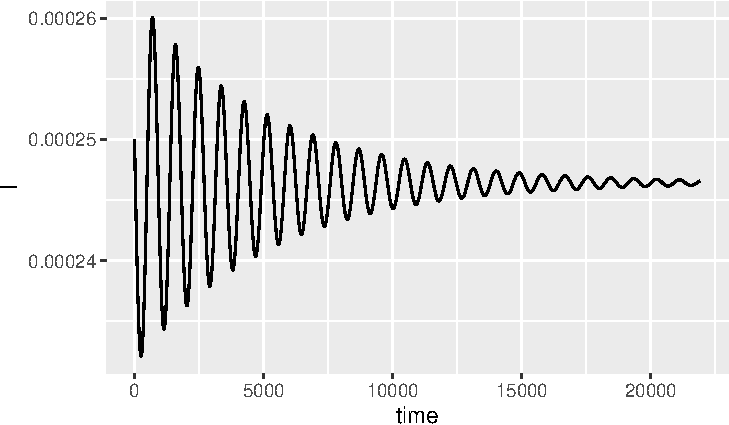
\includegraphics{Analisis-estabilidad_files/figure-beamer/unnamed-chunk-4-1.pdf}
\end{frame}

\hypertarget{resultado-1}{%
\subsection{Resultado}\label{resultado-1}}

\begin{frame}{Resultado}
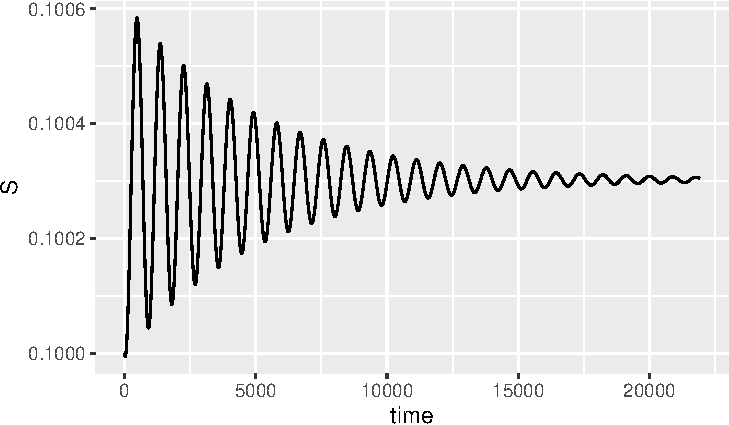
\includegraphics{Analisis-estabilidad_files/figure-beamer/unnamed-chunk-5-1.pdf}
\end{frame}

\hypertarget{actividad}{%
\section{Actividad}\label{actividad}}

\begin{frame}{Actividad}
Calcula de las condiciones de equilibrio endémico con los valores de los
parámetros utilizados
\end{frame}

\hypertarget{un-marco-muxe1s-generalizable-para-el-anuxe1lisis-de-estabilidad}{%
\section{Un marco más generalizable para el análisis de
estabilidad}\label{un-marco-muxe1s-generalizable-para-el-anuxe1lisis-de-estabilidad}}

\hypertarget{la-matriz-jacobiana-j}{%
\subsection{\texorpdfstring{La matriz Jacobiana
(\(J\))}{La matriz Jacobiana (J)}}\label{la-matriz-jacobiana-j}}

\begin{frame}{La matriz Jacobiana (\(J\))}
\begin{equation}
J = \left[
\begin{matrix}
\frac{\partial f^*_1}{\partial N_1} & \frac{\partial f^*_1}{\partial N_2} & \dots & \frac{\partial f^*_1}{\partial N_n} \\

\frac{\partial f^*_2}{\partial N_1} & \frac{\partial f^*_2}{\partial N_2} & \dots & \frac{\partial f^*_2}{\partial N_n} \\

\vdots & \ddots & & \vdots \\

\frac{\partial f^*_n}{\partial N_1} & \frac{\partial f^*_n}{\partial N_2} & \dots & \frac{\partial f^*_n}{\partial N_n} \\
\end{matrix}
\right]
\end{equation}
\end{frame}

\hypertarget{desmenuzando}{%
\subsection{Desmenuzando}\label{desmenuzando}}

\begin{frame}{Desmenuzando}
\begin{itemize}
\item
  \(f^*_1 \rightarrow \dot{S} = 0\)
\item
  \(f^*_2 \rightarrow I^*\)
\item
  \(f^*_3 \rightarrow R^*\)
\item
  \(\partial S^* / \partial S\) quiere decir que es una derivada parcial

  \begin{itemize}
  \tightlist
  \item
    Se calcula igual, pero se considera que todo lo demás es constante
  \end{itemize}
\end{itemize}
\end{frame}

\hypertarget{obteniendo-las-derivadas-parciales}{%
\subsection{Obteniendo las derivadas
parciales}\label{obteniendo-las-derivadas-parciales}}

\begin{frame}{Obteniendo las derivadas parciales}
\[S^* = \mu - \beta S^*I^* - \mu S^*\]

Si sólo consideramos que \(S\) es una variable:

\[\frac{\partial S^*}{\partial S} = -\beta I^* - \mu\]
\end{frame}

\hypertarget{obteniendo-las-derivadas-parciales-1}{%
\subsection{Obteniendo las derivadas
parciales}\label{obteniendo-las-derivadas-parciales-1}}

\begin{frame}{Obteniendo las derivadas parciales}
En la derivada parcial con respecto de \(I\), tratamos a \(S\) como
constante y a \(I\) como variable:

\[\frac{\partial S^*}{\partial I} = -\beta S^*\]

Y en la de \(R\), \(S\) e \(I\) son constantes

\[\frac{\partial S^*}{\partial R} = 0\]
\end{frame}

\hypertarget{la-matriz-completa-una-vez-que-calculamos-todas-las-parciales}{%
\section{La matriz completa una vez que calculamos todas las
parciales}\label{la-matriz-completa-una-vez-que-calculamos-todas-las-parciales}}

\hypertarget{matriz-j-de-sir}{%
\subsection{\texorpdfstring{Matriz \(J\) de
\(SIR\)}{Matriz J de SIR}}\label{matriz-j-de-sir}}

\begin{frame}{Matriz \(J\) de \(SIR\)}
\begin{equation}
J = \left[
\begin{matrix}
-\beta I^* - \mu & - \beta S^* &  0 \\
\beta I^* & \beta S^* - (\gamma + \mu) & 0 \\
0 & \gamma & -\mu
\end{matrix}
\right]
\end{equation}
\end{frame}

\hypertarget{quuxe9-se-hace-con-j}{%
\subsection{\texorpdfstring{Qué se hace con
\(J\)}{Qué se hace con J}}\label{quuxe9-se-hace-con-j}}

\begin{frame}{Qué se hace con \(J\)}
\begin{itemize}
\item
  Para encontrar cómo se llegará al equilibrio endémico, calculamos los
  valores propios (\(\lambda_J\))
\item
  Si tenemos 3 compartimentos, habrá 3 valores propios
\item
  \(\lambda\) puede ser complejo, (p.~ej.
  \(\lambda = 1 - 3\sqrt{-1} = 1-3i\))
\item
  Si \(\lambda \in \mathbb{Z} \rightarrow\) se llegará al equilibrio
  endémico por medio de oscilaciones
\item
  Si la parte real de \(\lambda < 0\) el sistema eventualmente se
  equilibrará
\end{itemize}
\end{frame}

\hypertarget{ejercicio-2}{%
\section{Ejercicio 2}\label{ejercicio-2}}

\begin{frame}{Ejercicio 2}
Sustituye los parámetros en \(J\) y calcula los valores propios (puedes
usar cualquier herramienta).
\end{frame}

\hypertarget{para-finalizar}{%
\subsection{Para finalizar}\label{para-finalizar}}

\begin{frame}{Para finalizar}
\begin{itemize}
\item
  Las funciones \(f^*\) para \(J\) pueden ser cualesquiera
\item
  Método se puede aplicar para todo tipo de infecciones en una población
\item
  Otras cantidades importantes a calcular son la \textbf{edad promedio
  de primera infección} cuando la infección es endémica

  \begin{itemize}
  \tightlist
  \item
    Expresión derivada de \(J\) se puede utilizar en análisis de datos
    provenientes de poblaciones
  \end{itemize}
\end{itemize}
\end{frame}

\hypertarget{literatura}{%
\subsection{Literatura}\label{literatura}}

\begin{frame}{Literatura}
Keeling y Rohani (2007). Modeling Infectious Diseases in Humans and
Animals. Princeton (en existencia en la biblioteca).
\end{frame}

\end{document}
